%!TEX root = ../thesis.tex
%*******************************************************************************
%****************************** Third Chapter **********************************
%*******************************************************************************
\chapter{Physics of Liquid Argon Time Projection Chambers}
\label{Chapter3}
% **************************** Define Graphics Path **************************
\ifpdf
    \graphicspath{{Chapter3/Figs/Raster/}{Chapter3/Figs/PDF/}{Chapter3/Figs/}}
\else
    \graphicspath{{Chapter3/Figs/Vector/}{Chapter3/Figs/}}
\fi

%********************************** %Opening  **************************************

The Liquid Argon Time Projection Chamber (LArTPC) stands as a high precision detector in neutrino physics.
In contrast to liquid scintillator neutrino experiments, LArTPCs collect both light and charge thereby providing a superior granularity for imaging neutrino interactions.
The detector concept was first proposed in 1977 by Rubbia \cite{Rubbia}, bringing together the time projection chamber technology developed by Nygren \cite{Nygren1, Nygren2} and the liquid argon ionisation chamber developed by Willis and Radeka \cite{WillisRadeka}.
LArTPC provides excellent spatial, calorimetry and timing resolution while enabling a high neutrino interaction rate.
Thus, this novel technology remains the primary choice for many neutrino experiments at Fermilab.

%overview
The following chapter will delve into the operating principles of a LArTPC, which is the detection technology employed by the Short-Baseline Near Detector to be discussed in the forthcoming Chapter \ref{ChapterDetector}.
Section \ref{sec3:overview} provides an overview of the design of a LArTPC and the choice of liquid argon.
In Section \ref{sec3:creation}, a comprehensive discussion is presented on particle interactions with the liquid argon and the production of ionisation electrons and scintillation photons, which are the observables of a LArTPC.
Following that, Section \ref{sec3:propagation} outlines the propagation of the resultant electrons and photons through the liquid argon medium.
Section \ref{sec3:detection} provides an insight into the detection mechanism of the ionisation electrons and scintillation photons using wire planes and novel optical detection technologies respectively.
Finally, Section \ref{lartpcConclude} concludes the chapter with some remarks.

%********************************** %First Section  **************************************
\section{Overview of LArTPCs}
\label{sec3:overview}
%1: Introduction
The Liquid Argon Time Projection Chamber (LArTPC) is the technology of choice for Fermilab's neutrino program, due to its ability to facilitate a high rate of neutrino interactions while maintaining an exceptional spatial, energy, and timing resolution. 
Moreover, the abundance and low cost of argon are ideal for scaling detectors to a large target mass, reaching up to tens of kilotons of liquid argon.
Notably, the Short-Baseline Neutrino (SBN) programme \cite{SBNProgram} comprises three LArTPC experiments each of size in the hundreds of tons, located along the Booster Neutrino Beam (BNB): the Short-Baseline Near Detector (SBND) \cite{sbnd_det}, MicroBooNE \cite{ubooneDet}, and ICARUS \cite{icarus_det}.
This novel technology will also be utilised at the upcoming long baseline Deep Underground Neutrino Experiment (DUNE), of which two of the four far modules are LArTPCs, each with a volume of 17 kilotons \cite{dunefd_det}.

%2: LArTPC description and figure
Fig. \ref{fig:LARTPC} shows a diagram illustrating a general LArTPC.
The TPC comprises a volume of LAr with a uniform electric field provided by a surrounding field cage, which is not shown in the diagram.
To the right of the TPC is a cathode grounded at a high negative voltage and to the left is the anode plane assembly, and thus the resulting electric field direction is from left to right.
The anode plane assembly is made up of three wire planes oriented at different angles, of which the diagram here shows three planes at the angle of $0^{\circ}$ and $\pm60^{\circ}$ to the vertical.
Behind the wire planes is the Photon Detection System (PDS) comprising 9 PhotoMultiplier Tubes (PMTs).   

The centre of the LArTPC in Fig. \ref{fig:LARTPC} also depicts an example interaction of an incoming neutrino scattering off an argon nucleus, shown as the dashed line since the neutral track of the neutrino is unobservable by the detector.
Charged particles resulting from the neutrino interaction ionise and excite argon atoms as they traverse through the detector medium, producing ionisation electrons and scintillation photons in the process as shown by the solid lines.
Ionisation electrons drift towards the anode in the opposite direction of the electric field.
Upon arrival at the anode, ionisation electrons induce signals on the two inner wire planes and are collected on the outermost wire plane.
The combination of signals from the three planes results in a high granularity three-dimensional image of the charged particle path.
Moreover, since the wire planes are transparent to scintillation photons, the photons drift past the wire planes and are detected by the PDS.
Scintillation photons provide additional information about the deposited energy and precise timing information of the neutrino interaction.

\begin{figure}[ht!] 
\centering    
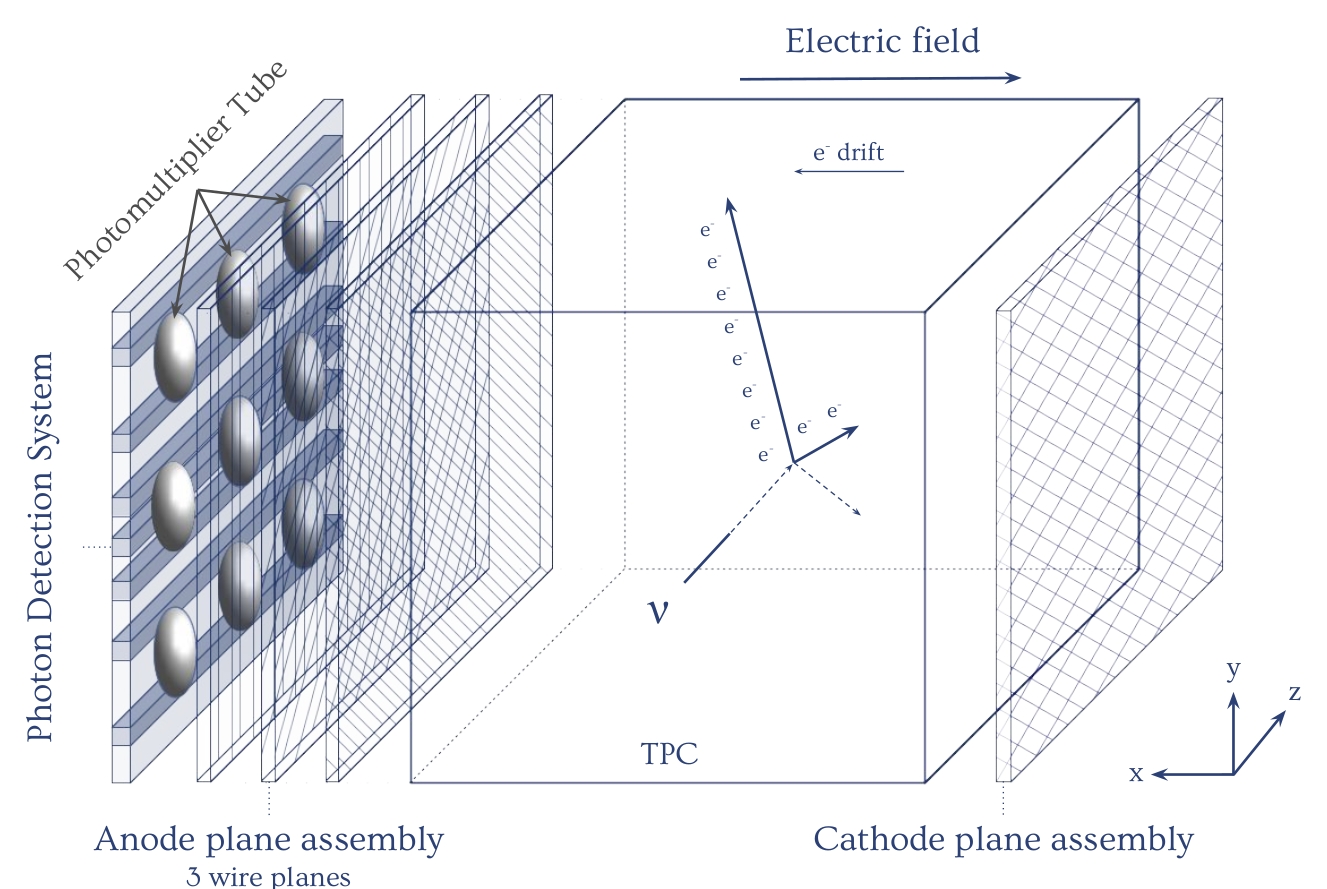
\includegraphics[width=0.95\textwidth]{LARTPC}
\caption[Liquid Argon Time Projection Chamber Diagram]{
Diagram illustrating the operating principles of a LArTPC \cite{RhiannonPhD}.
}
\label{fig:LARTPC}
\end{figure}

\newpage
%add why argon as target material
Liquid argon makes an excellent medium for TPCs in neutrino experiments.
Given that liquid argon has a reasonably high density of 1.39 g$\cdot$cm$^{-3}$ and an atomic mass of 40, it enables a high rate of neutrino interactions since the probability of neutrino interactions increases with the number of nucleons in the detector volume.
Furthermore, given that argon is a noble element, most of the energy deposited by particles traversing through the medium is used for ionising and exciting atoms, producing ionisation electrons and scintillation photons in the processes.
This maximises the efficiency of energy transfer into observable signals as well as enables a low energy threshold for detection in the order of $\mathcal{O}$(10) MeV.
In addition to argon being an abundant and cheap material for scaling the detector target mass, recent technology advancements in purifying liquid argon have resulted in a stable and pure liquid argon condition for LArTPC operation.
This ensures that observable signals from electrons and photons can traverse the drift distance towards detection without being captured by contaminants \cite{ubooneEtime}.
Consequently, liquid argon continues to stand out as an advantageous target material for neutrino experiments. 

%Additionally, liquid argon has a very high electron mobility, allowing for ionisation electrons to quickly drift under an electric field.

\section{Particle Interactions in Liquid Argon}
\label{sec3:creation}

Particle interactions in liquid argon and the production of ionisation electrons and scintillation photons as observable signals are discussed in the following section.       
Section \ref{sec3:bethebloch} provides a description of the energy loss of charged particles traversing liquid argon and producing ionisation electrons.                          
Following that, Section \ref{sec:scintillation} details the production mechanism of scintillation photons via excitation and recombination.                                       
Finally, Section \ref{sec:recomb} goes into more detail of the physics of recombination that determines the yield of ionisation electrons and scintillation photons.

%Ionisation
\subsection{Production of Ionisation Electrons}
\label{sec3:bethebloch}

%Energy loss profile
Charged particles traversing a medium, such as liquid argon, undergo energy loss via ionisation, producing electrons.                                                                       
The typical energy loss profile is illustrated in Fig. \ref{fig:BetheBloch}, specifically for a muon traversing in a copper medium; however, the underlying principle applies to liquid argon.
The plot depicts the stopping power, which is the energy loss per unit length divided by the density of the target medium, against the momentum of the traversing particle \cite{Passage}.
Heavy particles such as muons, pions, and protons, experience energy loss in liquid argon described by the Bethe-Bloch formalism \cite{Passage}.
For lighter and highly relativistic particles, such as > 100 MeV electrons in liquid argon, the primary mechanism for energy loss is through radiative effects.

%Track like
Muons, pions and protons interact electromagnetically with argon atoms as they propagate through liquid argon primarily via ionisation, freeing electrons along their trajectories.
These straight-line trajectories are referred to as \textit{tracks}.
The trajectories can also be deflected by many small angle scattering, a phenomenon known as Multiple Coulomb Scattering due to charged particles Coulomb scattering from nuclei \cite{Passage}. 
Within the momentum range of 1--100 MeV, the energy deposited per unit length via ionisation $dE/dx$ remains generally constant, often referred to as the Minimum Ionising Particle (MIP).
In this MIP region, the distribution of $dE/dx$ is described by a Landau-Gaussian convolution \cite{Passage}. 
When the particle comes to a stop, the deposited energy increases, forming the Bragg peak.
The energy loss profile described here is dependent on the mass of the traversing particle, making it a valuable tool for Particle IDentification (PID) \cite{argoneut}.
This method is the most effective for protons separation from muons and pions as protons are significantly heavier.

\begin{figure}[ht!] 
\centering    
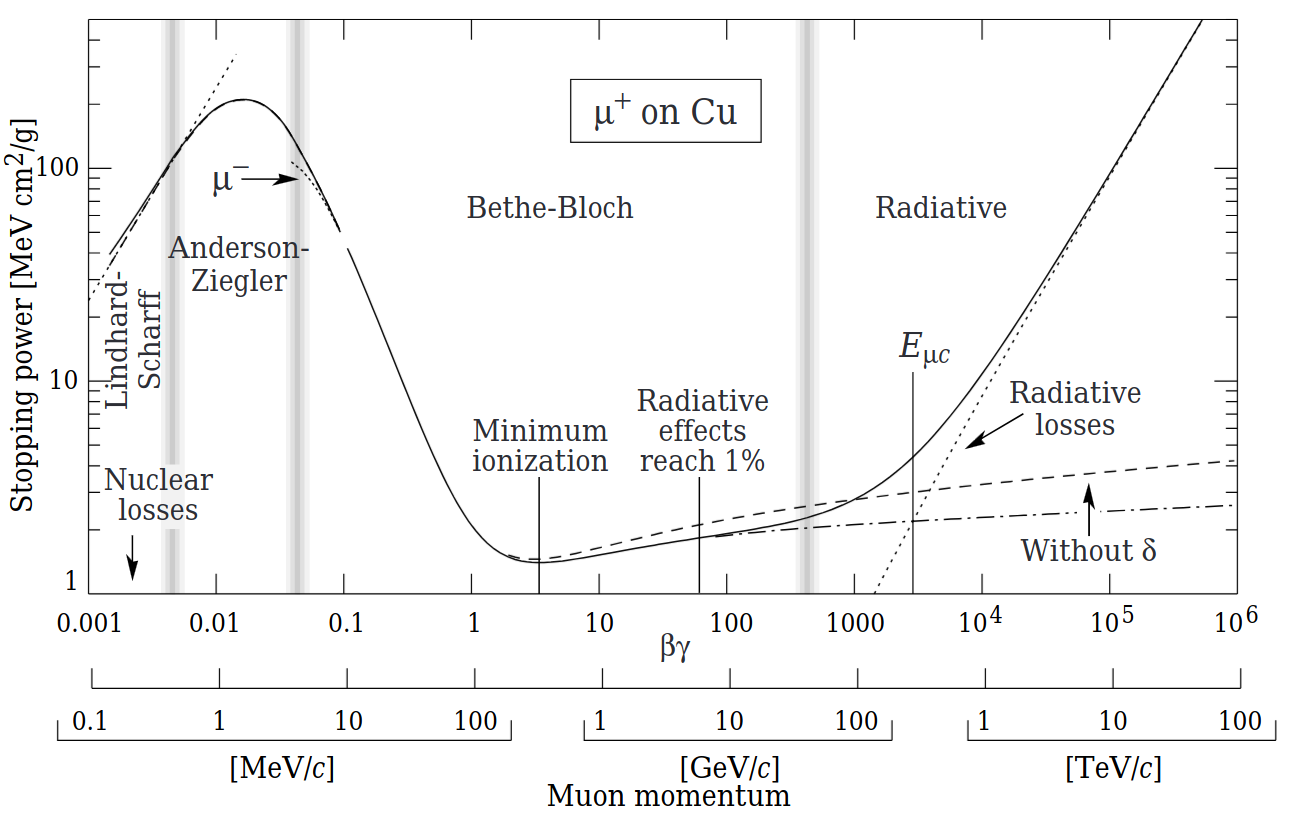
\includegraphics[width=0.95\textwidth]{BetheBloch}
\caption[Muon Energy Loss in a Copper Medium]{
Energy loss in matter for a muon traversing a copper medium \cite{Passage}.
}
\label{fig:BetheBloch}
\end{figure}

%Shower like
Electrons with energy above the critical energy, which is the point losses due to ionisation are equal to losses from radiation, deposit energy via radiative effects.
The critical energy for electrons in liquid argon is 39 MeV \cite{uboone_gamma}.
This process typically results in cones of electromagnetic activities, commonly referred to as \textit{showers}.
In the energy range relevant in a LArTPC, typically between 100--1000 MeV, showers deposit energy over a distance of $\sim$1 m, and the shower length is logarithmic in energy.
For electrons resulting from a muon decay with an energy of $\sim50$ MeV, they neither resemble an ionisation track nor an electromagnetic shower.
Instead, they result in a short linear segment of ionisation followed by a few clumps of deposited charge in the energy range of 1--10 MeV.
This unique energy deposition of electrons is referred to as a \textit{Michel electrons} and is often used by LArTPC experiments for energy calibration and identifying muons  \cite{uboone_michel}.

Photons deposit energy via Compton scattering and $e^+e^-$ pair production, also producing electromagnetic showers similar to energetic electrons.
Fig. \ref{fig:uboone_gamma} shows the mean free path of photons in liquid argon as a function of the photon energy for the two modes, Compton scattering by the solid blue line and pair production by 
the solid red line.
At the low energy range < 50 MeV, the main interaction mode is via Compton scattering while at the high energy range > 50 MeV, pair production becomes the dominant effect.
The mean free path for a photon for pair production is defined as 9/7 of the radiation length of an electron and it is plotted as the solid cyan line at 18.1 cm.
In the photon energy range of 100--1000 MeV relevant for LArTPCs, it can be seen that photons typically travel 20--30 cm without causing ionisation.
This creates a gap between the interaction vertex and the start of the shower, known as the \textit{conversion gap}.
Both the energy loss profiles and the conversion gaps can be utilised to distinguish between electrons and photons. 

\begin{figure}[ht!] 
\centering    
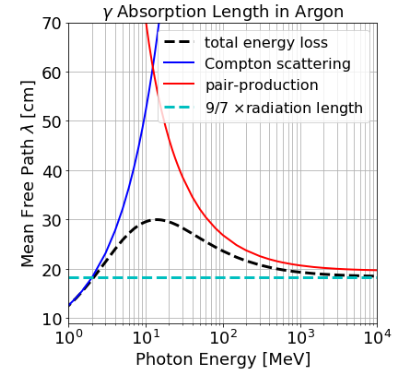
\includegraphics[width=0.5\textwidth]{uboone_gamma}
\caption[Mean Free Path of Photons in Liquid Argon]{
Mean free path of photons traversing in liquid argon as a function of their energies \cite{uboone_gamma}.
}
\label{fig:uboone_gamma}
\end{figure}

Fig. \ref{fig:track_shower} shows an event display of a simulated charged current $\nu_{\mu}$ interaction containing a muon, a proton and a neutral pion in the final state.
The colour scale corresponds to the magnitude of the energy deposition, where the colour green is lower in ionisation and the colour red is higher in ionisation.
The muon results in a long minimum ionising track whilst the proton results in a short energetic stub, demonstrating the distinct difference between the energy loss profile of a muon and a proton.
Moreover, as the muon comes to a stop, the colour scale changes from green to red, which indicates the increase in energy forming the Bragg peak.
At the end of the muon track, it decays into a Michel electron that resemblances a short linear segment low in energies. 
On the other hand, the neutral pion decays into two photons, which both undergo pair production producing electromagnetic showers.
The photon showers are detached from the interaction vertex where both muon and proton tracks begin.
This is the conversion gap feature unique to a photon shower.

\begin{figure}[ht!] 
\centering    
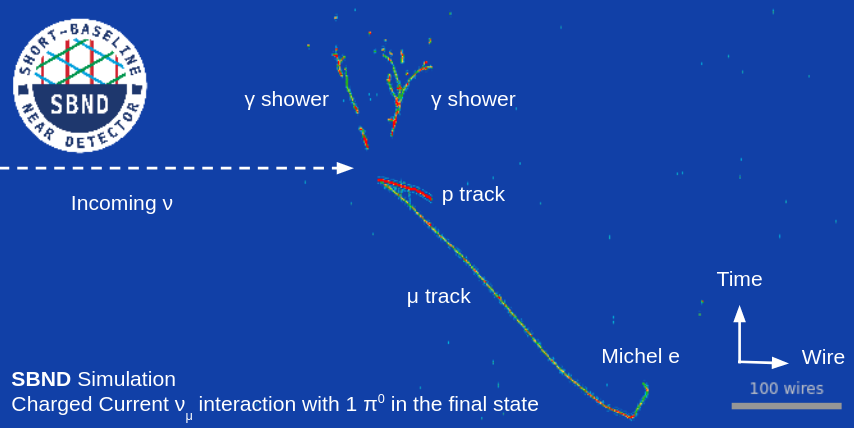
\includegraphics[width=0.85\textwidth]{event_display}
\caption[Event Display of a Neutrino Interaction]{
Event display showing a simulated charged current $\nu_{\mu}$ interaction containing a muon, a proton and a neutral pion in the final state.
}
\label{fig:track_shower}
\end{figure}

\subsection{Production of Scintillation Photons}

\label{sec:scintillation}

%Scintillation light
Charged particles traversing liquid argon also produce scintillation photons, through two different processes that result in an argon excimer $Ar_{2}^{*}$ as shown in Fig. \ref{fig:recomb_diagram}.  
The first process is known as recombination, denoted by the arrows labelled \textit{ionize} and \textit{recombine}.
Ionisation in liquid argon produces a free electron and an argon ion $Ar^{+}$.
The electron can either escape and drift towards the anode for detection, or recombine with an argon compound ion $Ar_2^{+}$, forming an argon excimer.
The second process is known as a self-trapped exciton, denoted by the arrow labelled \textit{excite}.
This begins when the charged particle does not have sufficient energy for ionisation, instead it excites the argon atom upon collision.
The excited argon atom $Ar^{*}$ self-traps with another argon atom $Ar$, forming an argon excimer.
The resulting argon excimer from both processes is short-lived and undergoes radiative decay into two ground-state argon atoms.
This produces scintillation photons with a wavelength of 128 nm in the Vacuum Ultraviolet (VUV) range \cite{Lariat}.

\begin{figure}[ht!] 
\centering    
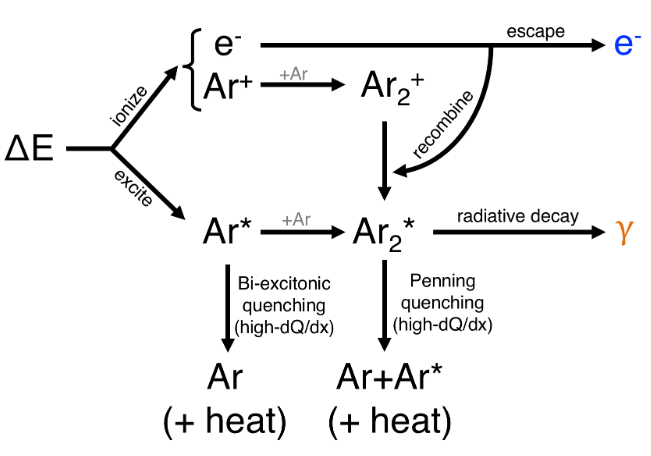
\includegraphics[width=0.55\textwidth]{recomb_diagram}
\caption[Energy Deposition in Liquid Argon Diagram]{
Production of ionisation electrons and scintillation photons from energy deposition processes in liquid argon \cite{Lariat}.
}
\label{fig:recomb_diagram}
\end{figure}

The timing constant of the radiative decay depends on the excitation state of the argon excimer.
This can be either a singlet state where the excited electron has the same spin as in the ground state or the triplet state where the excited electron has the same spin as another unpaired electron.
The singlet state has a shorter mean lifetime with a decay constant $\tau_{1} \approx 6 - 7$ ns, while the triplet state has a longer mean lifetime with a decay constant $\tau_{3} \approx 1.5 - 1.6$ 
$\mu$s \cite{photon_lifetime}.
These are referred to as the prompt and or late components, respectively. 
The time-dependent probability of light emission in pure liquid argon is modelled as:
\begin{equation}
        l(t)=\frac{A_{1}}{\tau_{1}}\exp{\left(-\frac{t}{\tau_{1}}\right)} +\frac{A_{3}}{\tau_{3}}\exp{\left(-\frac{t}{\tau_{3}}\right)},
\end{equation}
where $A_{1}$ and $A_{3}$ are the decay amplitudes of the singlet and triplet state.

%Quenching
Liquid argon serves as an excellent medium for producing scintillation photons, such that the light yield is as high as $\sim$40,000 photons per MeV of deposited energy in the absence of an electric field \cite{light_yield}.
In a typical electric field at 500 V/cm, as configured in SBND, the light yield decreases to $\sim$20,000 photons per MeV of deposited energy due to free electrons being drifted before recombination can occur \cite{light_yield_Efield}.
Furthermore, high ionisation density may lead to non-radiative quenching effects \cite{Lariat}.
Contaminants in liquid argon, such as oxygen and nitrogen, can absorb energy from argon excitons and excimers, without emitting any photons.
 
\subsection{Recombination}
\label{sec:recomb}

%Recombination
The electron-ion recombination, as depicted by the arrow labelled \textit{recombine} in Fig. \ref{fig:recomb_diagram}, is a key physics process affecting the yield of ionisation electrons and scintillation photons.
Recombination occurs almost immediately within 1-2 ns following the ionisation process.                                                                                                                
The recombination factor $R$ is defined as the survival probability of electrons that do not recombine.
Fig. \ref{fig:recomb_graph} shows a comparison of various $R$ models with a non-linear dependence on the energy density $dE/dx$ for liquid argon at an electric field of 500 V/cm \cite{argoneut_recomb}.
The Birks model, shown by the solid blue line, has been disfavoured due to spurious values at high charge density.
The Box model, shown by the solid red line, is based on the columnar theory around the charge deposition and can resolve the issue suffered by the Birks model.
It has been recently modified for better agreement with the Birks model at low charge density which accounts for the presence of an electric field and local ionisation density.
The modified Box model, as shown by the dotted red line, also contains experimentally derived parameters measured by the ArgoNeuT experiment \cite{argoneut_recomb}.

%, and formally modelled as follows \cite{argoneut_recomb}
%\begin{equation}
%	R=W_{ion} \cdot \frac{dE/dx}{dQ/dx}
%	\label{eq:recomb}
%\end{equation}
%where $W_{ion} = 23.6$ eV is the energy required to ionise an argon \cite{ion_e} and $dQ/dx$ and $dE/dx$ is the charge and energy loss per unit length respectively. 

\begin{figure}[ht!] 
\centering    
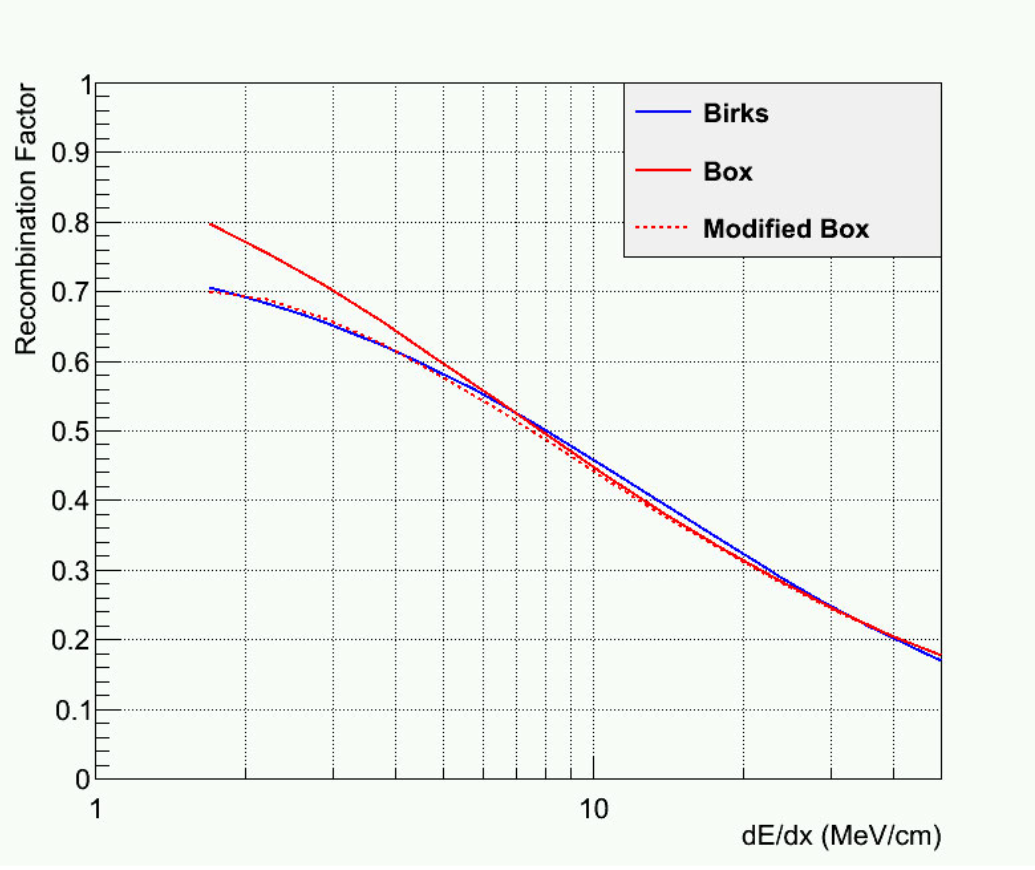
\includegraphics[width=0.6\textwidth]{recomb_graph}
\caption[Reombination Factor in Liquid Argon]{
Recombination factor in liquid argon as a function of the deposited energy density for an electric field of 500 V/cm \cite{argoneut_recomb}.
}
\label{fig:recomb_graph}
\end{figure}

%A popular model to describe this effect is the Box Model, based on columnar theory around the charge deposition \cite{box_model}. 
%The inverse Box Model equation is formulated as \cite{argoneut_recomb}
%\begin{equation}
%	\frac{dE}{dx} = \frac{1}{\beta}\left[ \exp{\left( \beta W_{ion}  \frac{dQ}{dx}\right)} -\alpha \right]
%\end{equation}
%where $\alpha$ and $\beta$ are experimentally derived parameters.
%Recombination is highly dependent on the electric field and the local charge density, which is folded into the $\beta$ parameter.
%ArgoNeuT experiment recently conducted a data-driven study on recombination in LArTPC, resulting in the ``Modified Box Model" with parameter $\alpha = 0.93$ and $\beta = 0.30 $ MeV/cm \cite{argoneut_recomb}.
%If not taken into account, the recombination can result in underestimating energy loss due to ionisation.

The dependence of recombination on the electric field leads to an anti-correlation between the charge and light yield $Q$ and $L$ respectively, such that \cite{argoneut_recomb}:
\begin{gather}
        \label{eq:Q}
        Q = N_{i}R, \\ 
        \label{eq:L}
        L = N_{ex} + N_{i}(1 - R),
\end{gather}
where $N_{i}$ is the number of electron-ion pairs and $N_{ex}$ is the number of argon excitons.
Fig. \ref{fig:QLAnti} illustrates the anti-correlation as a function of the electric field strength for various noble elements, of which argon is shown as dashed lines.
A stronger electric field results in a higher number of ionisation electrons being separated from the argon ions and drifting towards the anode for detection before recombination can occur, thus increasing the charge yield. 
Conversely, scintillation photons are produced in the recombination process.
In the presence of an electric field, recombination decreases, leading to a reduction in light yield.
Furthermore, the recombination factor can be influenced at a local scale due to ionisation density resulting from interacting particles.
The SBND detector operates with an electric field of 500 V/cm, a region where the energy deposition to ionisation electrons and scintillation electrons are approximately equal as can be seen in Fig.
 \ref{fig:QLAnti}.
The impact of recombination on the observed physics will be further discussed in Chapter \ref{ChapterCalib}, Section \ref{sec7:delta}.

\begin{figure}[ht!] 
\centering    
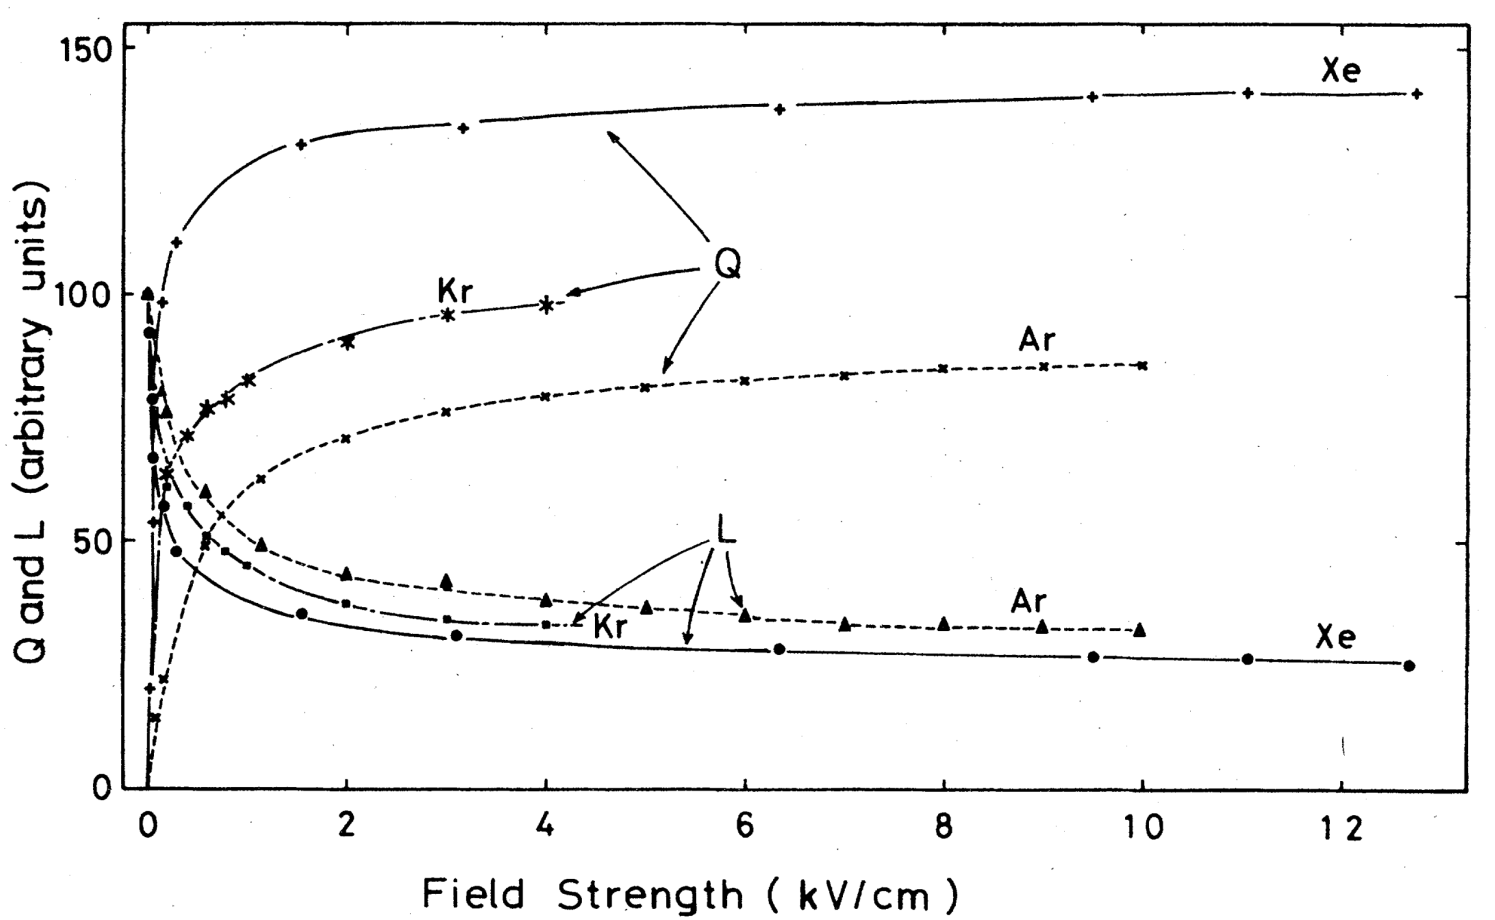
\includegraphics[width=0.85\textwidth]{QLAnti}
\caption[Charge and Light Yield as a Function of Electric Field]{
Anti-correlation of charge yield $Q$ and light yield $L$ as a function of the electric field strength \cite{QLAnti}.
}
\label{fig:QLAnti}
\end{figure}

\section{Particle Propagation in Liquid Argon}
\label{sec3:propagation}

The following section provides a description of the transportation of ionisation electrons and scintillation photons through the liquid argon medium.
Section \ref{sec:edrift} covers the details of different physics processes that electrons experience as they drift towards the anode, including diffusion, attenuation and the space charge effect.
On the other hand, a discussion on the propagation of photons is presented in Section \ref{sec:photonprop}, detailing the process of Rayleigh scattering, absorption and wavelength shifting.

%Transportation of ionised electrons, diffusions, impurities
\subsection{Electron Drift}
\label{sec:edrift}

%\subsubsection{Diffusion}

%Electron drift under electric field
Ionisation electrons that do not recombine drift towards the anode under the effect of an electric field.
In a typical LArTPC with an electric field of 500 V/cm and a temperature of 88.4 K, the drift velocity of electrons is approximately 0.156 cm/$\mu$s \cite{drift_vel}.
As the electrons drift, they undergo diffusion, causing perturbations in their trajectories due to various effects.
For example, it can be due to inelastic collisions with argon atoms.
Diffusion causes the shape of a cloud of electrons produced in a point-like energy deposition to grow in volume while drifting.
The effects increase with the drift distance, smearing both spatial and temporal resolutions. 

Diffusion is parameterised in both the longitudinal and the transverse direction, which are parallel and perpendicular to the drift direction respectively.
Longitudinal diffusion affects the temporal resolution, as individual electrons arrive at the wire either earlier or later relative to the electron cloud moving at the average drift velocity.
The temporal smearing due to the longitudinal diffusion can be approximated as \cite{uboone_diff}:
\begin{equation}
        \sigma_{L} \approx \sqrt{\frac{2D_L}{v^{2}_{d}}t},
\end{equation}
where $D_L$ (cm$^2$/s) is the longitudinal diffusion, $v_{d}$ (cm/s) is the drift velocity and $t$ (s) is the drift time.
%$D_L$, in this case, is an effective longitudinal diffusion coefficient containing a small contribution from transverse diffusion \cite{uboone_diff}.
On the other hand, transverse diffusion broadens the cross section of the electron cloud arriving at the original wire, causing electrons to migrate to neighbouring wires.
The spatial smearing due to the transverse diffusion can be approximated as \cite{GrayDiffusion}:
\begin{equation}
        \sigma_T \approx \sqrt{2 \cdot D_T \cdot t},
\end{equation}
where $D_T$ (cm$^2$/s) is the transverse diffusion and $t$ (s) is the drift time.
Collectively, both longitudinal and transverse diffusion smear the distribution of deposited energy seen by each wire, thereby impacting the measured energy loss profile of a particle \cite{GrayDiffusion}.
At the conditions expected for the SBND detector, the diffusion coefficients have been measured to be $D_{L} = 4.0 $ cm$^{2}$/s at the MicroBooNE detector \cite{uboone_diff} and $D_T = 8.8 $ cm$^{2}$/s \cite{protodune}.

%\subsubsection{Attenuation}
%impurity: electron lifetime
In addition to diffusion, drifting electrons can also undergo attenuation.  
In this process, electrons are captured by electronegative impurities present in the liquid argon, most commonly oxygen and water \cite{protodune}.
This results in a reduction of electrons arriving at the wires, proportional to the drift distance. 
The number of charges collected on a wire $Q_{wire}$ is typically modelled as an exponential suppression:
\begin{equation}
	Q_{Wire} (t) = Q_{Dep} \cdot \exp\left(\frac{-t}{\tau}\right),
\label{eq:etime}
\end{equation}
where $Q_{Dep}$ is the original number of deposited charges, $t$ (ms) is the drift time and $\tau$ (ms) is the electron lifetime characterising the level of charge attenuation.
A high electron lifetime, resulting from a low level of contamination, is a critical operational factor for achieving high efficiency in energy reconstruction.
Recently reported from ProtoDUNE, which utilised the same membrane cryostat technology as SBND, the experiment measured a lifetime of $\sim$10 ms, equivalent to an oxygen purity of 3.4 ppt \cite{protodune}.
This lifetime is significantly larger than the drift time of SBND, which is projected to be 1.25 ms, making the effect of attenuation almost negligible. 

%Add how SBND measures electron lifetime and purification system (?)

%\subsubsection{Space Charge Effect}
%space charge effect

A final important issue in electron transport is the so-called Space Charge Effect (SCE).
Argon ions, produced as part of the ionisation process, drift towards the cathode at a slower velocity than electrons.
Typically, they have a drift velocity more than five orders of magnitude lower than that of electrons. \cite{icarus_sce}.
Since SBND is a surface detector without an overburden, high exposure to cosmic rays leads to a high rate of ionisation.
The resulting accumulation of slow-moving argon ions distorts the uniformity of the electric field, affecting both its intensity and direction.
Fig. \ref{fig:SCE} illustrates the deformation of tracks drifting in the distorted electric field due to SCE.
Track trajectories are impacted two-fold: bending away towards the detector edges as shown by the middle plot and bowing towards the cathode as shown by the right plot \cite{SCE}.
Moreover, distortions of the electric field also affect recombination previously discussed in Section \ref{sec:recomb}, since the recombination factor is dependent on the electric field strength.
Local fluctuations of recombination can subsequently impact the local charge yield resulting from an energy deposition.

\begin{figure}[htbp] 
\centering    
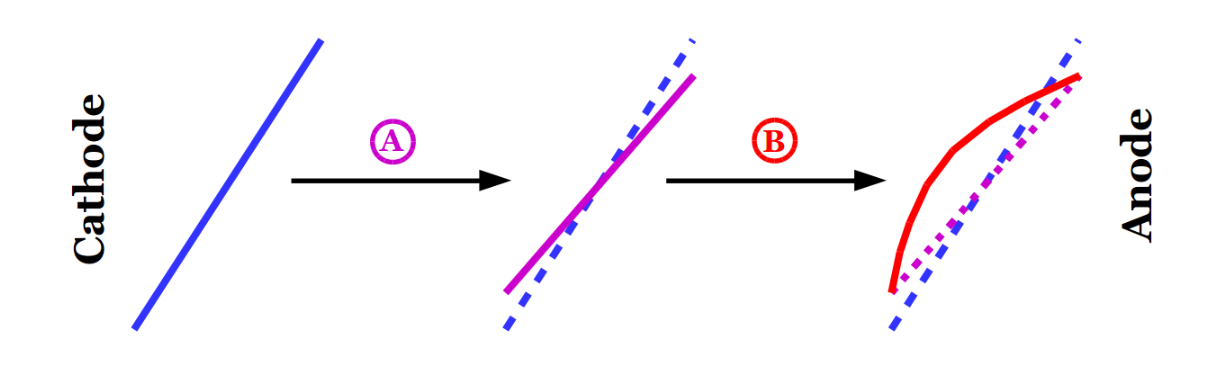
\includegraphics[width=0.85\textwidth]{SCE}
\caption[Impacts of Space Charge Effects on Tracks]{
Diagram showing the impacts of SCE on tracks: bending away towards the detector edges (middle) and bowing towards the cathode (right) \cite{SCE}.
}
\label{fig:SCE}
\end{figure}

%TODO: something sounds fudgy
%Therefore, SCE worsens the spatial as well as energy resolution of a track reconstruction and consequently, particle identification.
%SBND will implement a dedicated laser calibration system \cite{}, as well as calibration using cosmics track crossing cathode and anode \cite{} to model the distorted electric field.
%Once measured, correction will be applied in the reconstruction. 

\subsection{Photon Propagation}
\label{sec:photonprop}

%\subsubsection{Rayleigh Scattering}

%TODO: Check length, add group velocity/ rayleigh wavelength from Patrick's
Scintillation photons can propagate over long distances in liquid argon since the medium is transparent to its own light.
As scintillation photons travel, they undergo Rayleigh scattering as the first-order effect, involving the photons elastically scattering off atoms, altering their trajectories. 
Reflections and refractions at the boundaries of the detector material are second-order effects. 
While these effects do not change the number of photons, they modify the paths of propagation and lengthen the travel time \cite{sbnd_pds_paper}. 
The impact of these effects on the probability of photons reaching the Photon Detection System (PDS) depends on the locations where the photons are created and their paths taken to arrive at the PDS. 
This consequently leads to a non-trivial distribution of photon arrival time at the PDS, and the travel time can range from a few to several tens of nanoseconds.
Particularly, this effect is the most impactful on the prompt component of scintillation photons.
%, which is crucial for the purpose of triggering (See Chapter \ref{}) and high-precision timing analysis (see Chapter \ref{}).
The Rayleigh scattering length $\lambda_{RS}$ for VUV photons in liquid argon has been reported to be around 50 cm \cite{rayleigh50} up to 110 cm \cite{rayleigh110}, which is comparable to the size of SBND.

%\subsubsection{Absorption}

In addition to Rayleigh scattering, scintillation photons can also undergo absorption, which arises due to contaminants in liquid argon.
Contaminants like nitrogen \cite{photon_nitrogen} and methane \cite{photon_methane} have a high absorption cross section for VUV photons.
Other contaminants, like oxygen and water, have also been observed in commercial argon and can also attenuate the number of photons \cite{photon_commercial}. 
The absorption of scintillation photons is modelled as an exponential suppression similar to Eq. \ref{eq:etime} modelling the electron attenuation.
The number of photons surviving absorption $N_\gamma$ is as follows:
\begin{equation}
	N_{\gamma} (d) = N_0 \cdot \exp\left(\frac{-d}{\lambda_{A}}\right),
\label{eq:absorption}
\end{equation}
where $N_0$ is the original number of scintillation photons, $d$ is the propagation distance and $\lambda_A$ the absorption length.
Moreover, the absorption rate is dependent on the Rayleigh scattering length. 
Photons with a shorter $\lambda_{RS}$ undergo longer and more indirect paths, increasing their probability of absorption before reaching the PDS \cite{PatrickPhD}.

%\subsubsection{Wavelength Shifting}
%\label{sec:wls}


%Scintillation photons in the VUV range are typically absorbed by detector materials without being detected. 
Finally, an enhancement method for lighting collection efficiency in LArTPC is wavelength shifting scintillation photons.
Specifically at SBND, TetraPhenyl Butadiene (TPB) is employed to shift the wavelength of VUV photon from 128 nm to 430 nm, which falls within the visible light range.
This is to better match the detection spectrum of optical detectors installed at SBND \cite{sbnd_pds_paper}, of which a description of the SBND PDS will be detailed in Chapter \ref{ChapterDetector}.
Additionally, it provides extra handles for light reconstruction, of which the improvement will be discussed in Chapter \ref{ChapterReco}.

The propagation characteristics of photons differ between the VUV and visible range.
Fig. \ref{fig:vuv_visible} shows the group velocity on the left and the Rayleigh scattering length on the right as a function of the photon wavelength in liquid argon.
The vertical dashed blue and red lines at 128 and 430 nm respectively are the wavelengths of scintillation photons in liquid argon and of photons re-emitted by TPB wavelength shifting. 
Here, it can seen that the group velocity of VUV photons is slower than that of visible photons.
Moreover, the Rayleigh scattering length of VUV photons is two orders of magnitude smaller compared to visible photons.
This results in VUV photons being more susceptible to Rayleigh scattering and having a higher probability of absorption \cite{PatrickPhD}.

\begin{figure}[ht!] 
\centering    
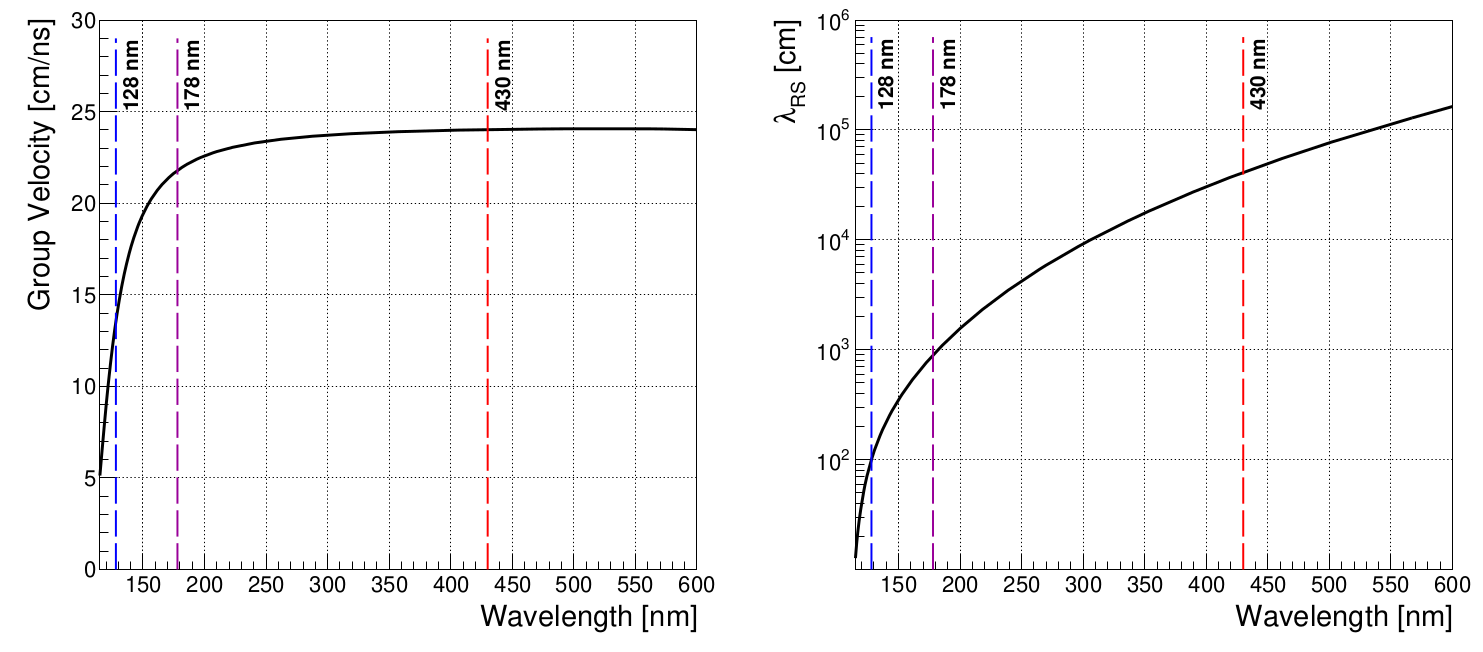
\includegraphics[width=1.0\textwidth]{vuv_visible}
\caption[Group Velocity and Rayleigh Scattering Length of Photons in Liquid Argon]{
Group velocity (left) and the Rayleigh scattering length (right) as a function of the photon wavelength in liquid argon \cite{PatrickPhD}.
}
\label{fig:vuv_visible}
\end{figure}

\section{Detection Electrons and Photons}

\label{sec3:detection}

Upon arrival at the anode for detection, ionisation electrons and scintillation photons are read out by different detection technologies.
Ionisation electron signals are recorded by the wire planes, which will be detailed in the following Section \ref{sec:wire}.
Following that, Section \ref{sec:pmtarapuca} provides a description of two different types of optical detectors for detecting scintillation photons.

\subsection{Wire Planes}
\label{sec:wire}

Once arrive at the anode, ionisation electrons induce signals on the wire planes, which are made up of three planes separated by a few mm as previously depicted in Fig. \ref{fig:LARTPC}.
A bias voltage is applied to each wire plane to create a drift field across the three planes.
This allows for electron transparency for the two innermost planes, also referred to as induction planes, where drifting electrons induce bipolar signals on the wires.
The electrons are then collected on the outermost plane, producing a unipolar signal, hence, this plane is referred to as the collection plane.
Fig. \ref{fig:wire_current} shows an example of induced currents on a wire as a function of time.
Here, it can be seen a bipolar signal on an induction plane in red and a unipolar signal on a collection plane in blue.
The three planes are oriented at an angle of 60$^{\circ}$ with respect to each other, of which the diagram in Fig. \ref{fig:LARTPC} shows three planes at the angle of $0^{\circ}$ and $\pm60^{\circ}$ to the vertical.                                                                                                                                                                                          
While three-dimensional spatial reconstruction of a signal requires a minimum of at least two wire planes, many modern LArTPC experiments use all three planes to improve the spatial resolution \cite{argoneut, icarus_det, ubooneDet, sbnd_det, protodune, dunefd_det}.

\begin{figure}[ht] 
\centering    
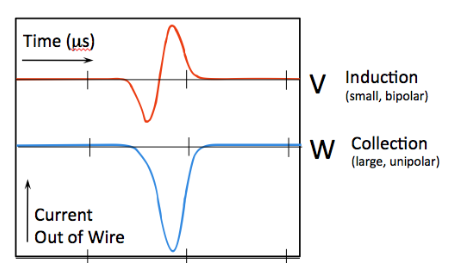
\includegraphics[width=0.57\textwidth]{wire_current}
\caption[Induced Currents on an Induction and a Collection Wire Plane]{
Current signals on the induction and collection wire plane induced by a point-like charge deposition \cite{argoneut}.
\hfill
\break
}
\label{fig:wire_current}
\end{figure}

%The signals induced or collected on the wire planes are then shaped, amplified, and digitized by cold electronics submerged in liquid argon to minimise noise.
%The data is then acquired by electronics locating outside of the cryostat. 

The signals induced or collected on the wire planes are then shaped, amplified, and digitized before acquisition.
Then, the measured signals are deconvolved for noise removal and the amount of charge collected is correlated with the energy deposited in the detector.
Finally, the reconstruction of spatial and energy information is performed, which allows for high level analysis like particle identification.
The reconstruction of charge signals at SBND will be further discussed in Chapter \ref{ChapterReco}, Section \ref{sec:reco_tpc}.

\subsection{Photomultiplier Tubes and X-ARAPUCAs}
\label{sec:pmtarapuca}

%Readout detection
Scintillation photons are detected by the PDS located behind the wire planes, as depicted in Fig. \ref{fig:LARTPC}. 
For SBND, which will detailed in the forthcoming Chapter \ref{ChapterDetector}, the primary detection technology in the PDS is Photomultiplier Tubes (PMTs), which have a Quantum Efficiency (QE) of up to 30\% \cite{pmt_qe}.
However, PMTs are typically large and require sufficient volume inside the detector for installation. 
Current and future LArTPC experiments are increasingly adopting Silicon PhotoMultipliers (SiPMs) due to their advantageous smaller size, lower power consumption, excellent signal-to-noise ratio, and a high QE of up to 40\% \cite{sipm_qe}.
The X-ARAPUCA device is a novel light collection technology utilising SiPMs, currently developed by Unicamp and being tested inside the SBND detector. 
Further description of X-ARAPUCA can be found in Ref. \cite{xarapuca}.

%As shown in Fig. \ref{fig:xarapuca}, it is a light guide designed to trap light through a combination of a wavelength shifter and dichroic filters.
%The dichroic filter is transparent to a narrow range of wavelengths and reflective otherwise, allowing only photons of specific wavelengths to pass through the filter and preventing their escape.
%The photons are internally reflected in the trap until they are detected by the SiPMs.
%The P-Therphenyl layer shifts 128 nm wavelength photons to 350 nm, allowing them to pass through the dichroic filter with a cut-off at 400 nm.
%The 350 nm photons are trapped inside the reflective cavity until detected by SiPM (right).
%The wavelength shifter plate converts the photons to 430 nm, trapping them by total internal reflection (left).
%
%\begin{figure}[htbp] 
%\centering    
%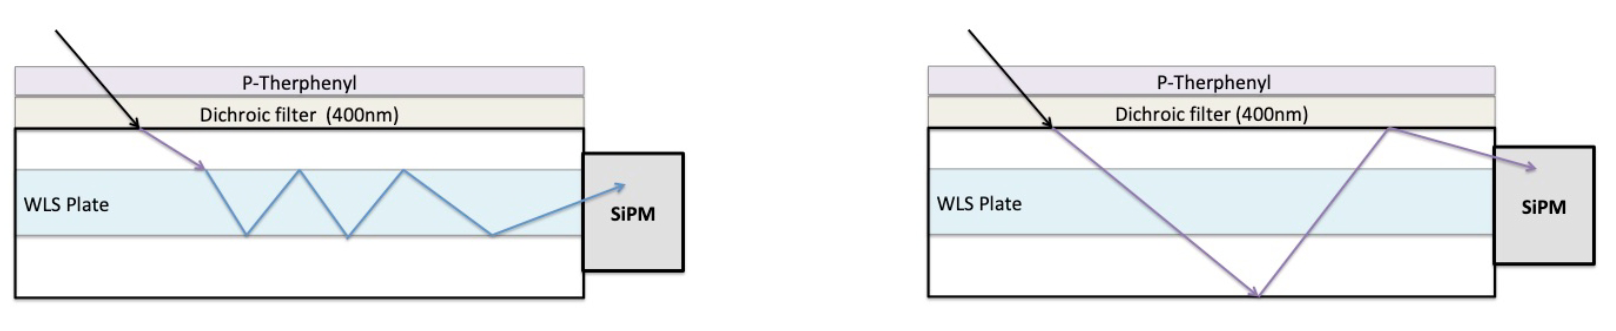
\includegraphics[width=1.0\textwidth]{xarapuca}
%\caption[xarapuca]{
%Diagram showing operating principles of a X-ARAPUCA \cite{xarapuca}.
%\hfill
%\break
%}
%\label{fig:xarapuca}
%\end{figure}

Both PMTs and X-ARAPUCAs are coated with wavelength shifting materials.
The re-emitted light direction is isotropic, causing coated optical detectors to suffer a 50\% reduction in efficiency due to photons being emitted away from the detection surface.
PMTs are coated specifically with TPB, which can also impact the detection time as the emission of visible photons is not instantaneous.
Multiple time components of re-emitted photons from TPB have been observed, with the majority of photons re-emitted within nanoseconds and a subset re-emitted as long as a few microseconds \cite{tpb_time}.

Photon signals measured by PMTs are digitized and acquired using a very high sampling frequency readout at the rate of 500 MHz \cite{sbnd_det}.
This high sampling frequency gives the scintillation light signal much better timing resolution compared to the charge signal.
As a result, it provides the most precise interaction timing information available in the detector.
This is particularly important across different areas of the SBND detector.
The PMT signals will be utilised for triggering which will be detailed in the forthcoming Chapter \ref{ChapterDetector}.
In addition, the signals enable the timing resolution of the light reconstruction to reach the order of $\mathcal{O}$(1) ns, which will be covered in Chapter \ref{ChapterReco}.
Then, the timing performance of the data acquisition to enable a stable and high frequency sampling of PMT signals will be further discussed in Chapter \ref{ChapterDAQ}.
All of these pave the way for the search for HNLs which is a key subject of this thesis, which will exploit the timing kinematic difference between HNL signals and SM neutrino backgrounds and will be covered in more detail in Chapter \ref{ChapterSelect} and \ref{ChapterResult}.

%********************************** %First Section  **************************************
\section{Concluding Remarks}
\label{lartpcConclude}
Since originally proposed in 1977, the LArTPC concept has proven its potential for use in precision neutrino experiments.
The understanding of particle interactions and their propagation within the detector, along with the detector's response to these particles, has significantly improved over time. 
Technological advancements in detection and readout now enable the scaling of LArTPCs from volumes of only several tons to even tens of kilotons, making them suitable for high multiplicity environments.
This allows for the next generation of LArTPCs like the DUNE experiment to advance the field of neutrino physics.
As described in the following Chapter \ref{ChapterDetector}, the SBND experiment and physics programme at Fermilab is a key part of this future.

